\message{ !name(ECE742Project.tex)}\documentclass{article}
\usepackage{amsmath}
\usepackage{mathtools}
\usepackage{graphicx}
\graphicspath{ {images/} }

\title{ECE 742 Final Project}
\author{
  Michelle King
  \and
  Suraj Suri
  }

\begin{document}

\message{ !name(ECE742Project.tex) !offset(300) }


 Some of these coefficients are identical, but we stored them separately for the
 purpose of organization and readable naming scheme.
 
\subsubsection{Graded PML}
The purpose of PML is to have the wave decay as the wave enters the PML, and a
nonzero conductivity value will achieve this decay. However, a large discrepancy
between the values of conductivity in the simulation region and the PML can
result in unwanted reflections.

The Reflection Factor is given by the equation:
\begin{equation}
  R(\theta)=\exp^{-2\eta cos(\theta)\int_{0}^{d}\sigma_{x}(x)dx
\end{equation}

  Where $\sigma_{x}$ is the graded conductivity of the PML material.\\
  $\theta$ is the angle of incidence of the wave. So steeper angles of $\theta$
  will result in higher values of reflection error.\\
  
We want to minimize reflection R but also make sure the wave decays completely
within the PML.

\subsubsection{Polynomial grading}
One type of grading, and the one  we have implemented, is the polynomial grading. We can
describe the grading in our code by the factors $\sigma$ and $\kappa$
Where the graded conductivity for the PML in the x direction is:
\[\sigma_{x} = (\frac{x}{d})^{m} \sigma_{x,max}\]
And the graded value for $\kappa$ for the PML in the x direction is:
\[\kappa_{x}=1+(\kappa_{x,max}-1)(\frac{x}{d})^{m}\]

We will vary the values for $\kappa_{max}$ and $\sigma_{max}$ in our numerical
experiments to test how different PML material conditions affect the
effectiveness of the PML.

An optimal expression for the value of $\sigma_{max}$ for a polynomial grading
has been found numerically to be:
\begin{equation}
\sigma_{x, optimal}=\frac{0.8(m+1)}{\eta_{0} \Delta x}
\end{equation}

\section{Experiment}
Each E and H 


\section{Error Analysis}
In order to test how well the PML is working to absorb the incoming reflection,
we will calculate the relative error with respect to the case of no boundary
conditions.

\begin{figure}
  \centering
  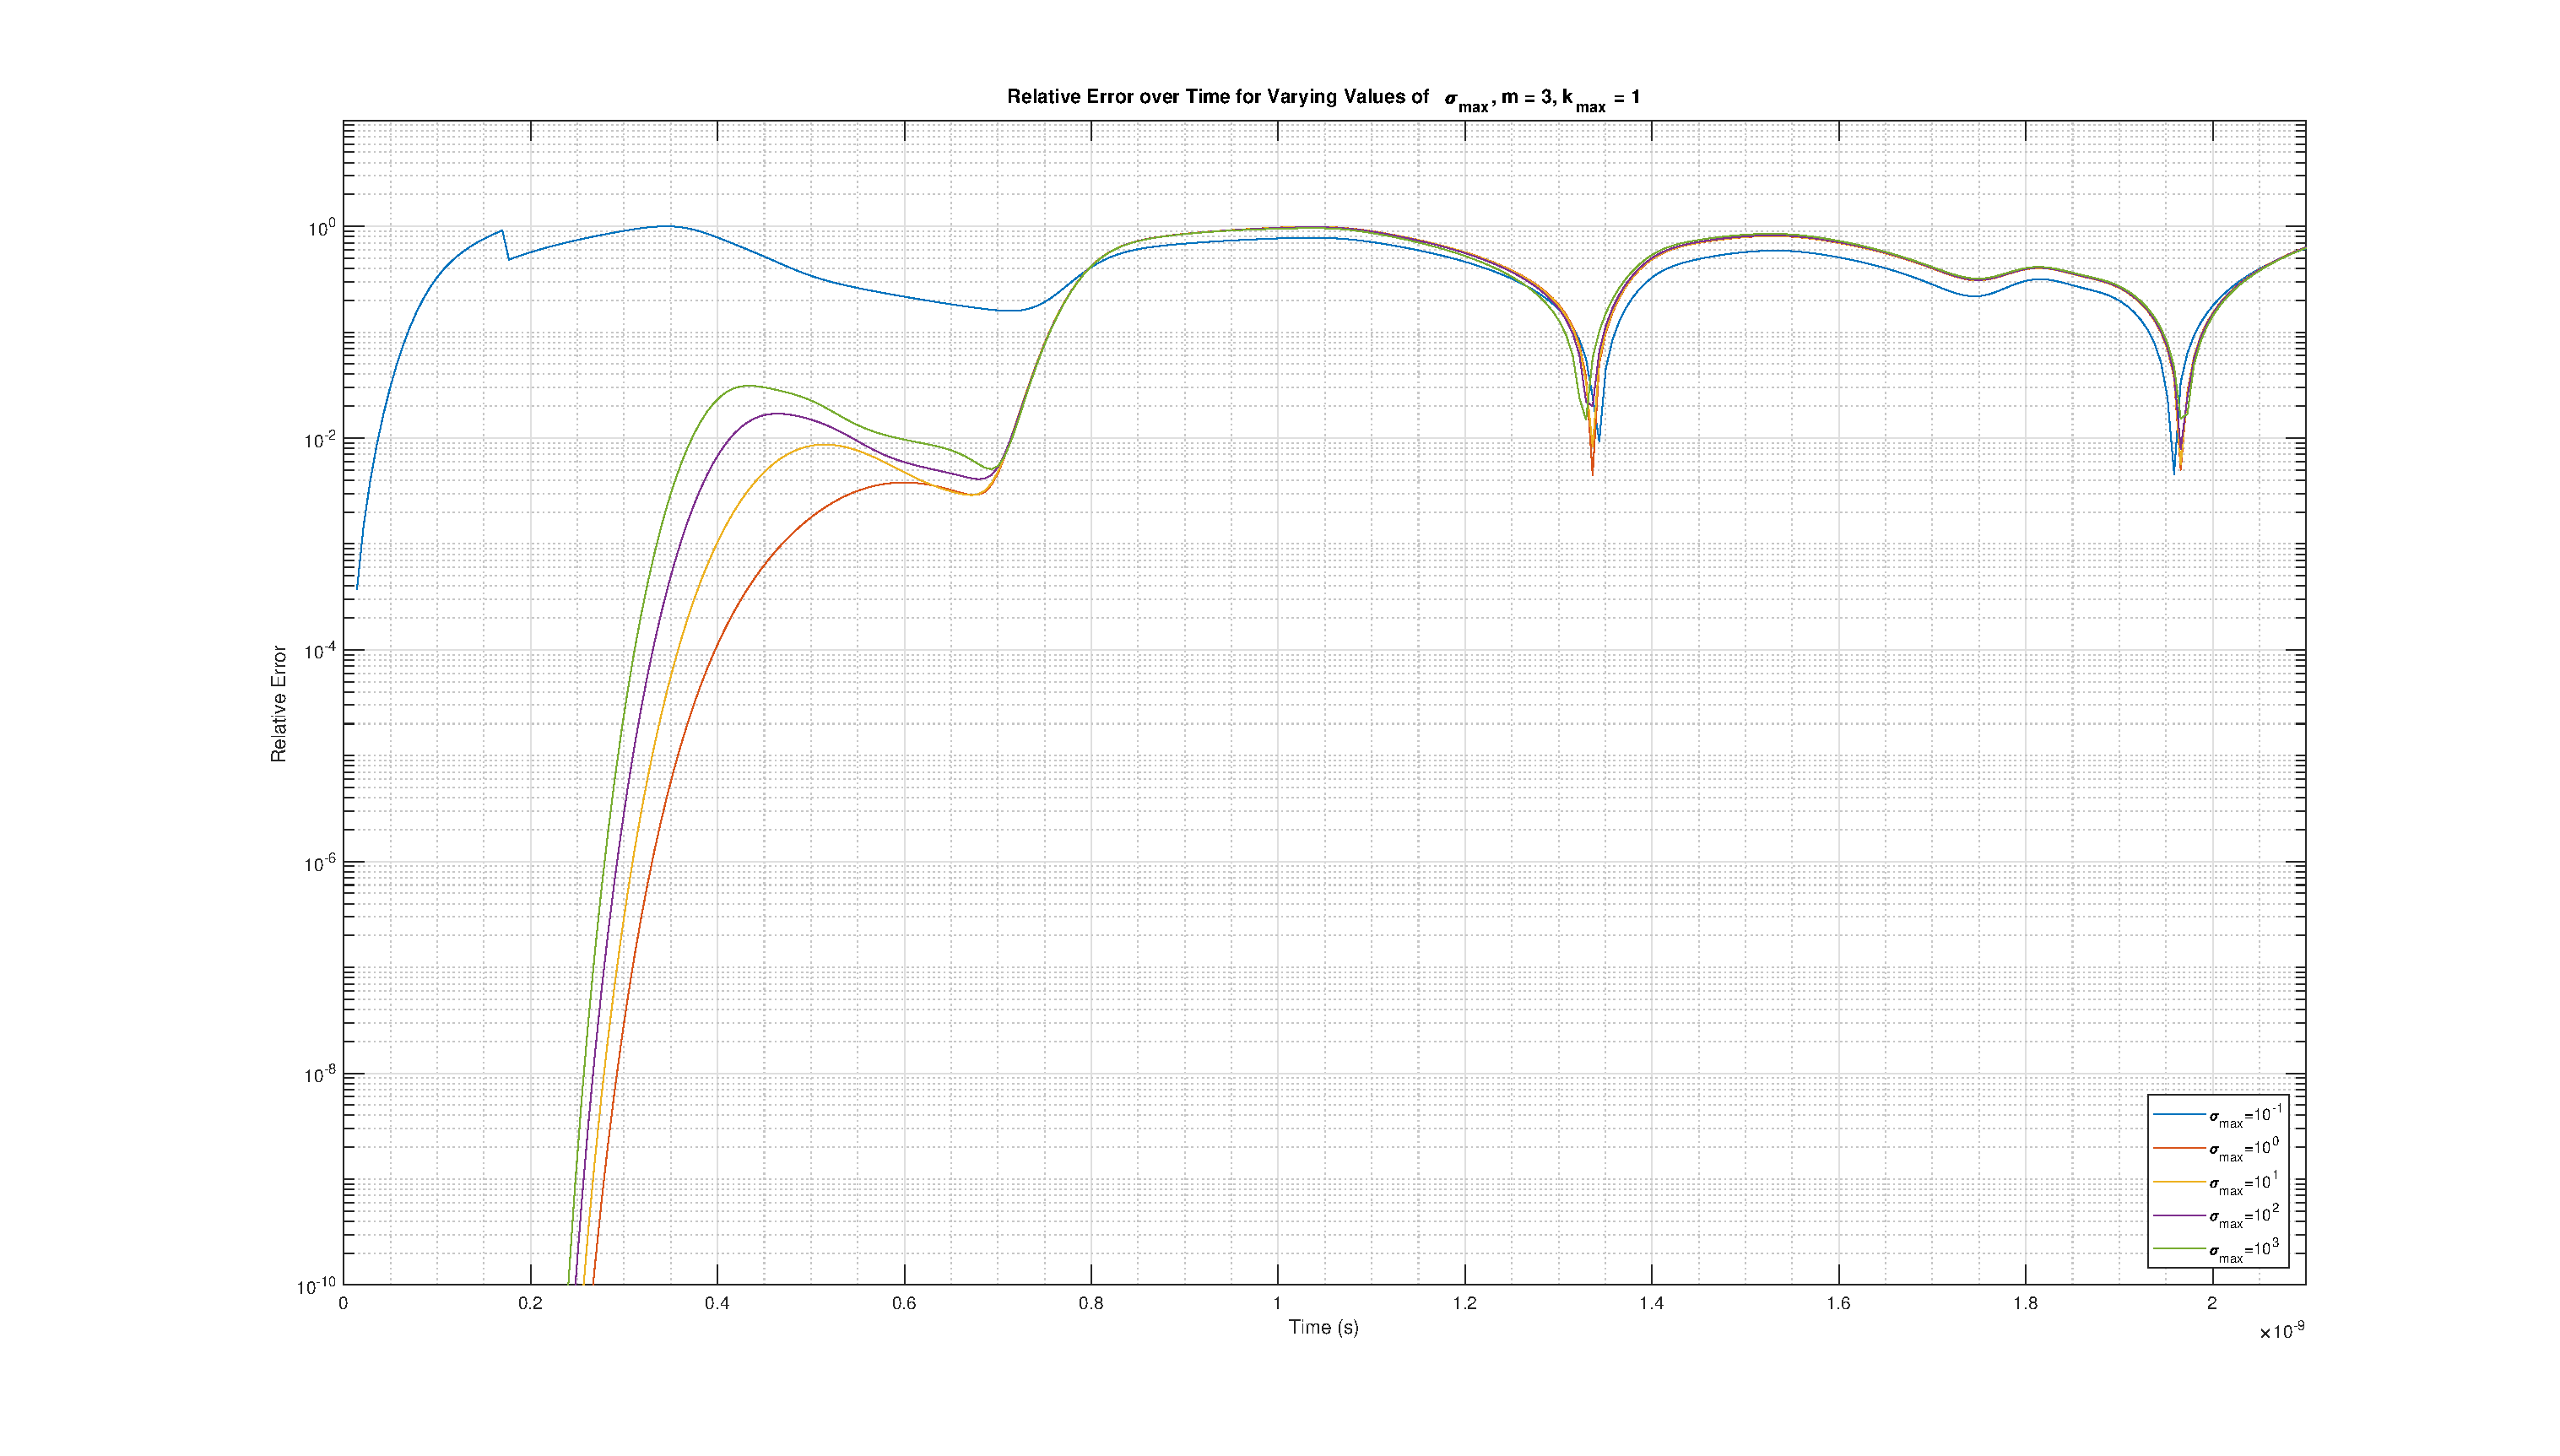
\includegraphics[width=\textwidth]{Rel_Err_SigMax_m3}
  \caption{Plot of ???}\label{fig:RelErrSigmaxm3}
\end{figure}

\begin{figure}
  \centering
  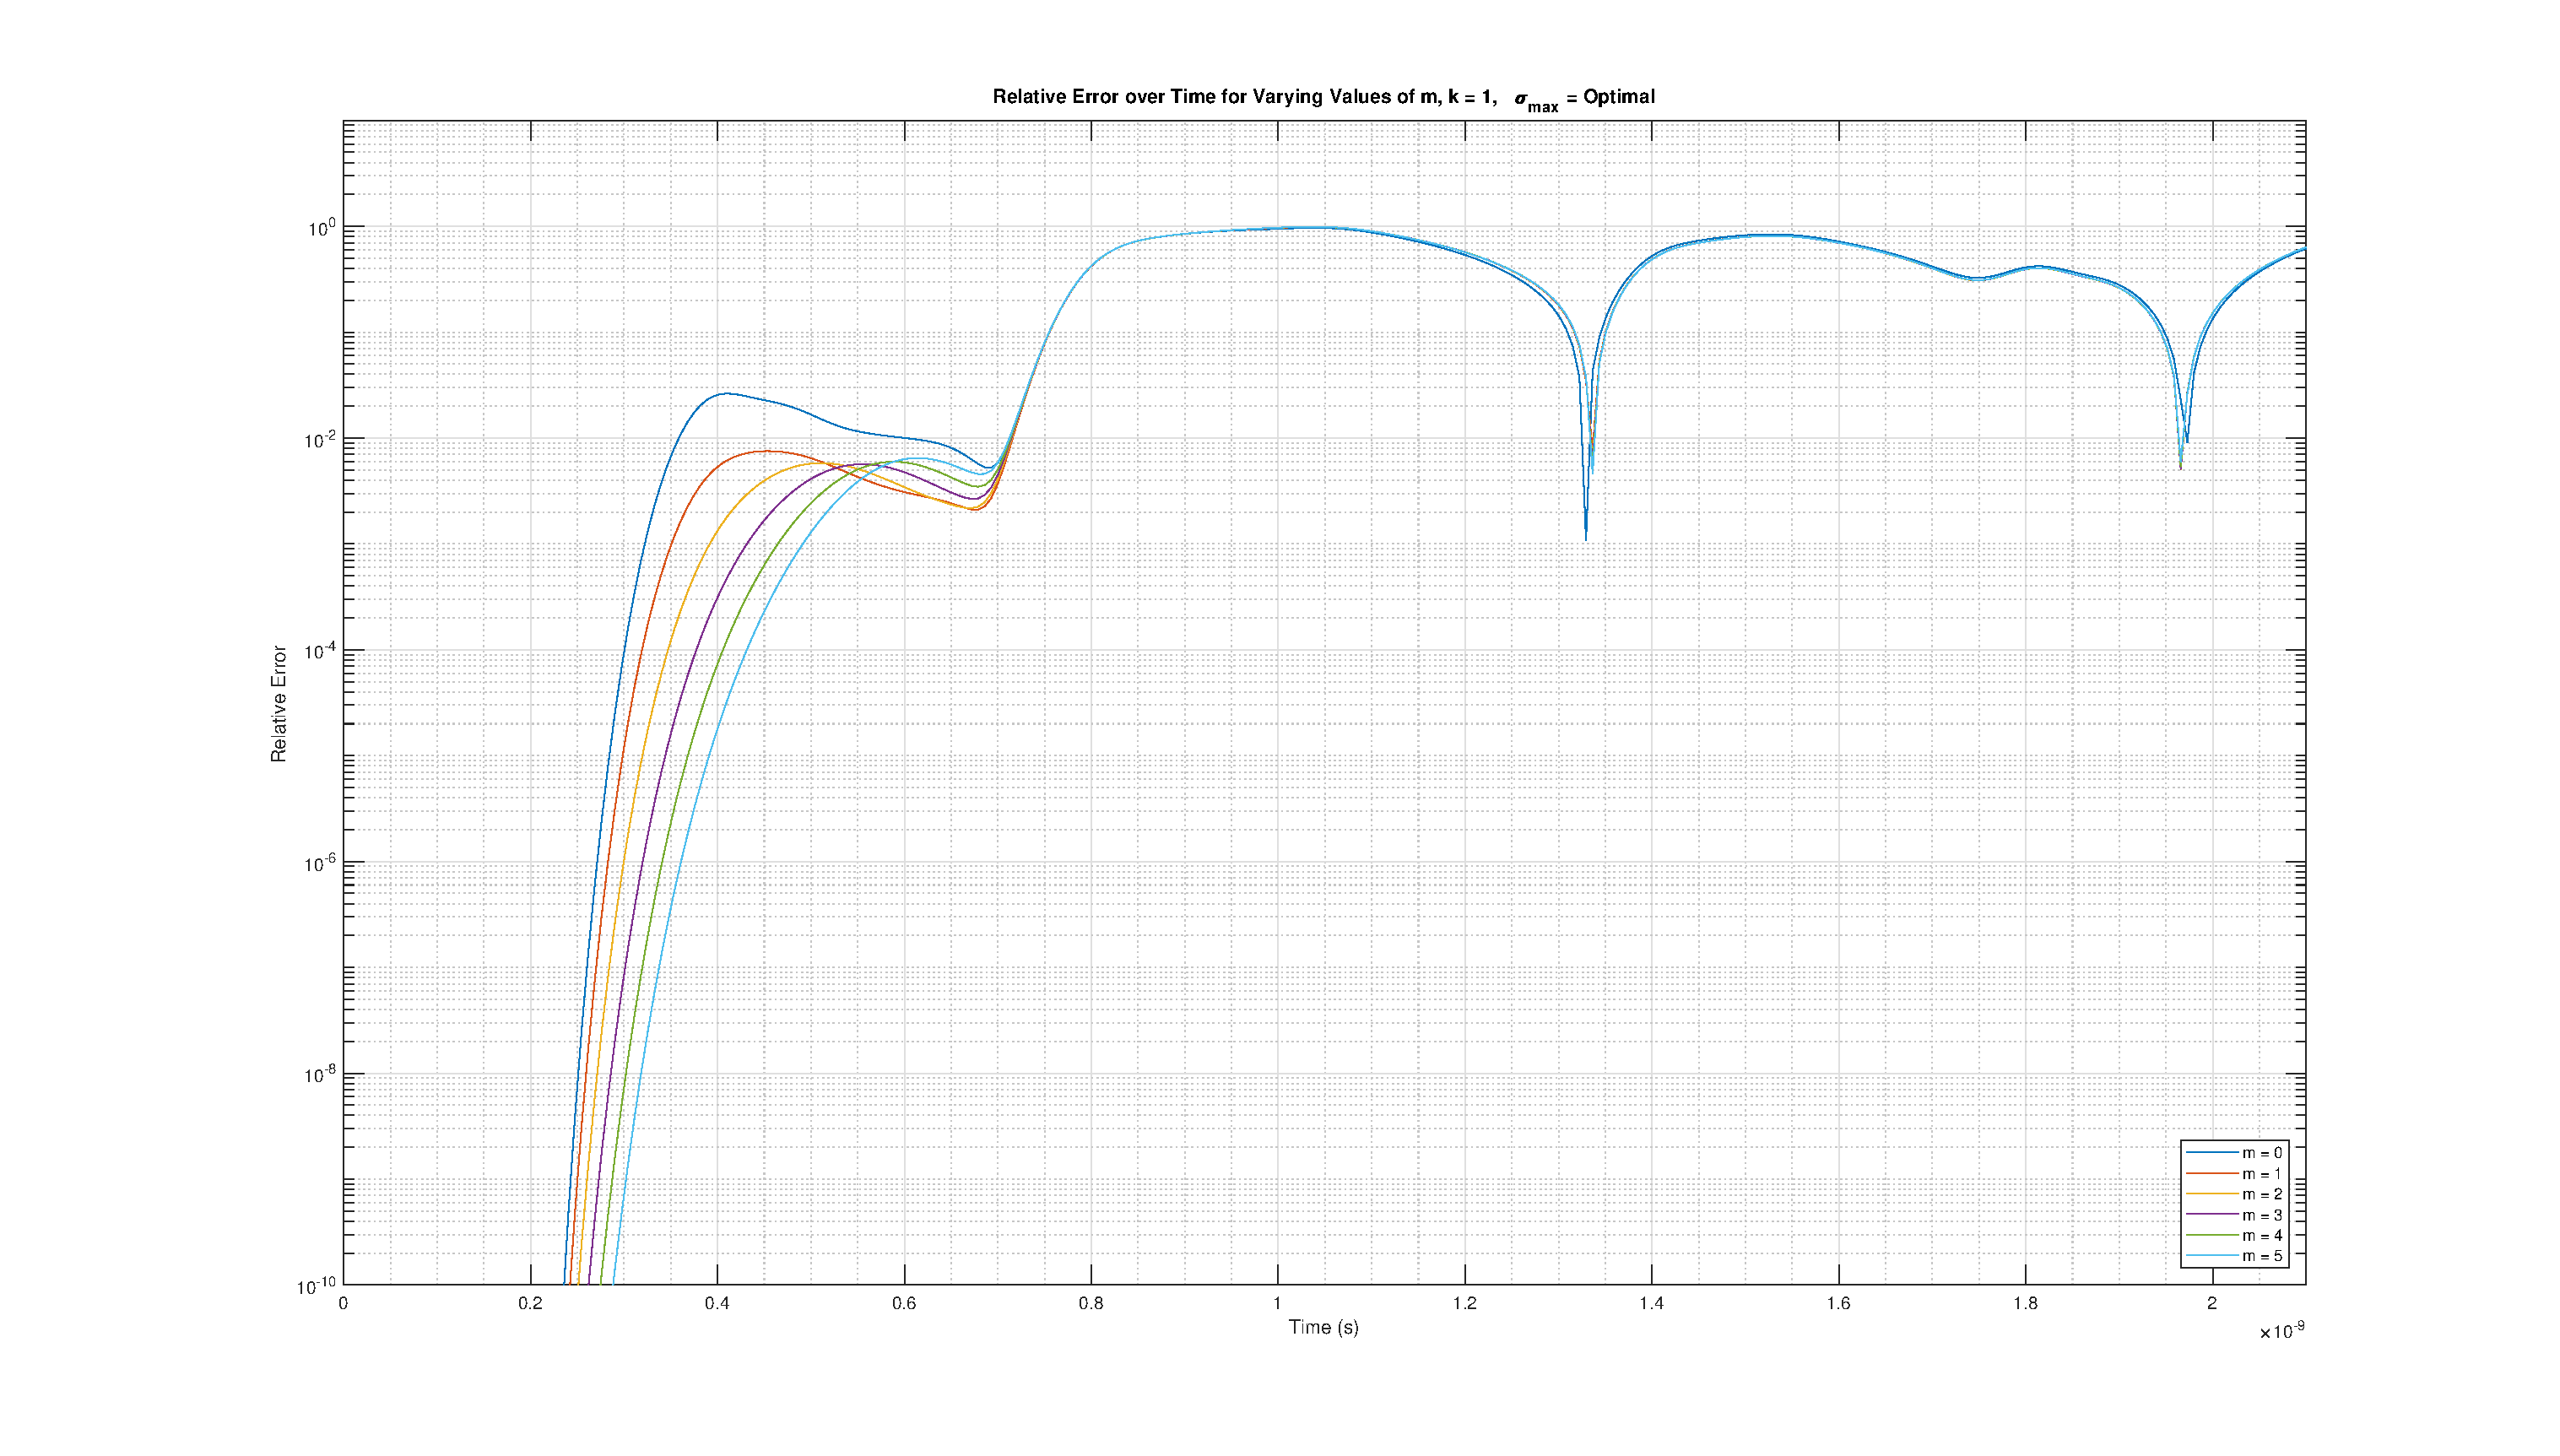
\includegraphics[width=\textwidth]{Rel_Err_m}
  \caption{Plot of ???}\label{fig:RelErrm}
\end{figure}

\begin{figure}
  \centering
  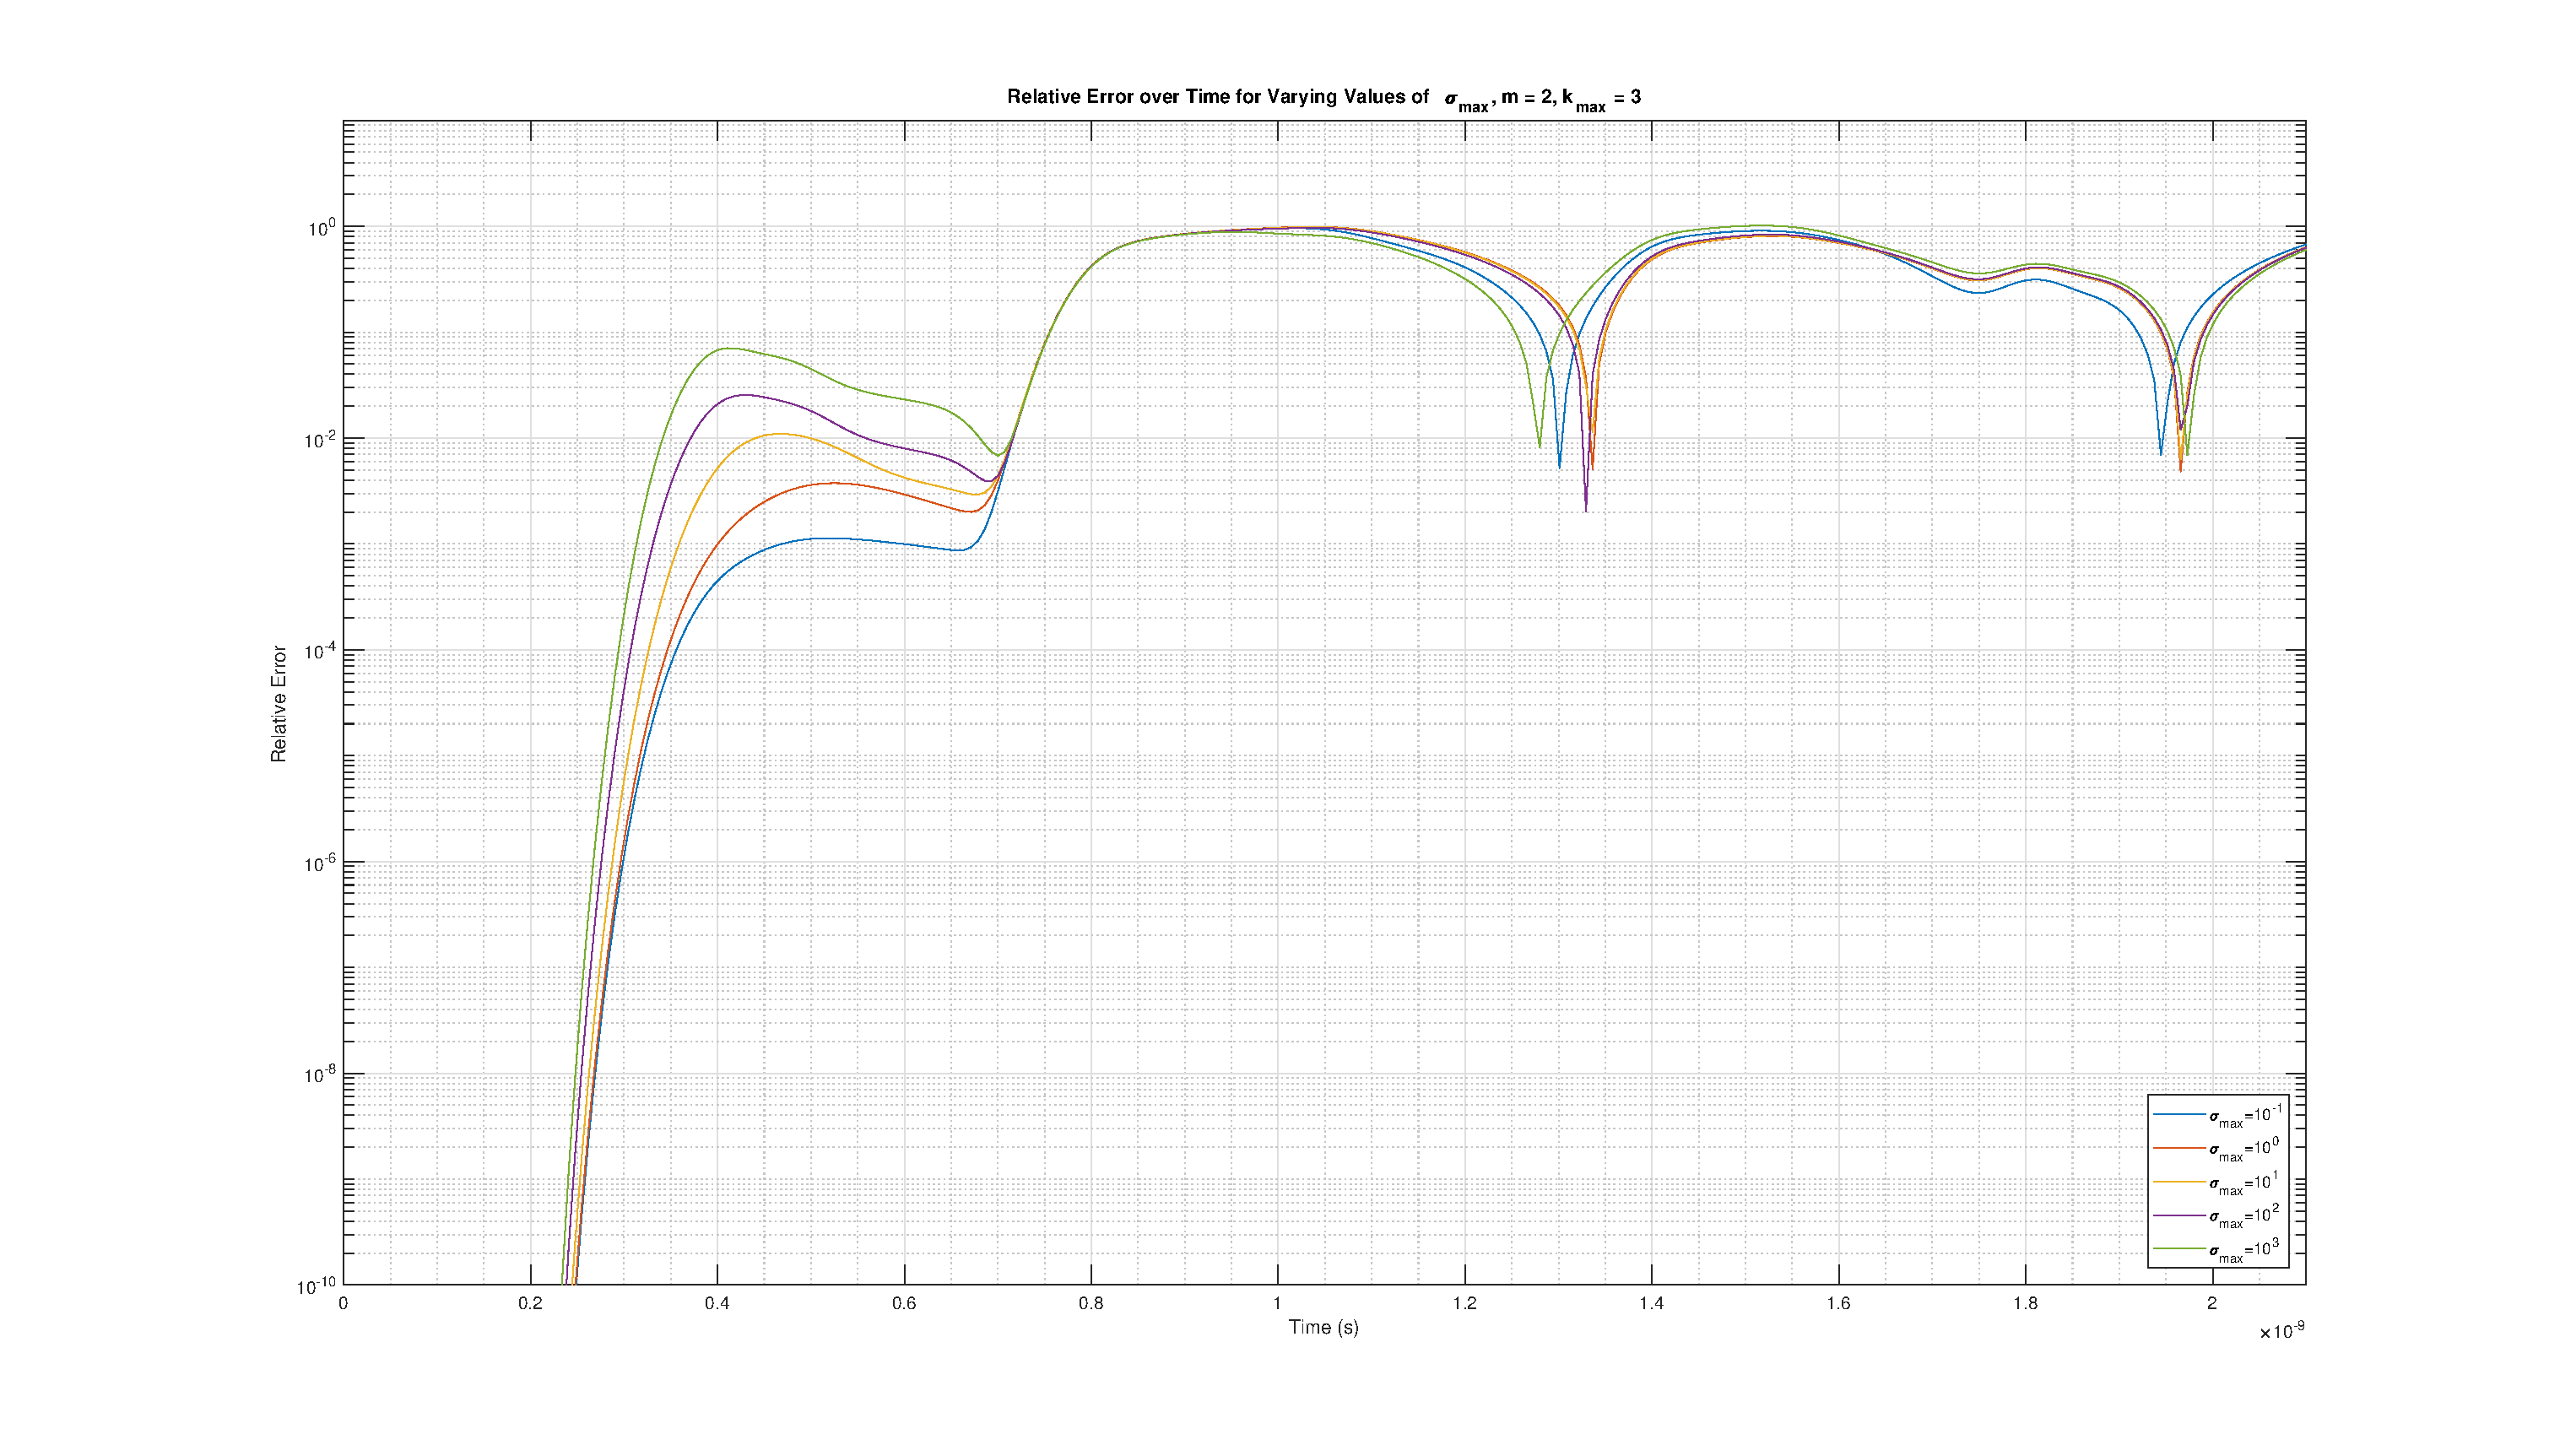
\includegraphics[width=\textwidth]{Rel_Err_SigMax}
  \caption{Plot of ???}\label{fig:RelErrSigmax}
\end{figure}

\section{Bibliography}
Followed Beringer's Derivation in Susan's book - third edition

\end{document}
\message{ !name(ECE742Project.tex) !offset(-89) }
